\documentclass[tikz,border=3pt]{standalone}
\usepackage[utf8]{inputenc}
\usepackage[T1]{fontenc}
\usepackage{lmodern}
\renewcommand{\familydefault}{\sfdefault}
\usepackage{sansmath}\sansmath
\usepackage{chemfig}
\usepackage{pgfplots}\pgfplotsset{compat=1.18,/pgf/number format/use comma,/pgf/number format/1000 sep={.}}
\usetikzlibrary{arrows.meta,calc,positioning,decorations.pathmorphing,patterns}
% paleta del sitio
\definecolor{nar}{HTML}{E8680C}\definecolor{narc}{HTML}{FFB35C}\definecolor{hielo}{HTML}{FFF3E8}
\definecolor{tinta}{HTML}{1D1D1F}\definecolor{gris}{HTML}{6E6E73}\definecolor{lila}{HTML}{7C5CF0}
\definecolor{azul}{HTML}{2F6FD6}\definecolor{menta}{HTML}{17A673}\definecolor{coral}{HTML}{E8342A}
\begin{document}
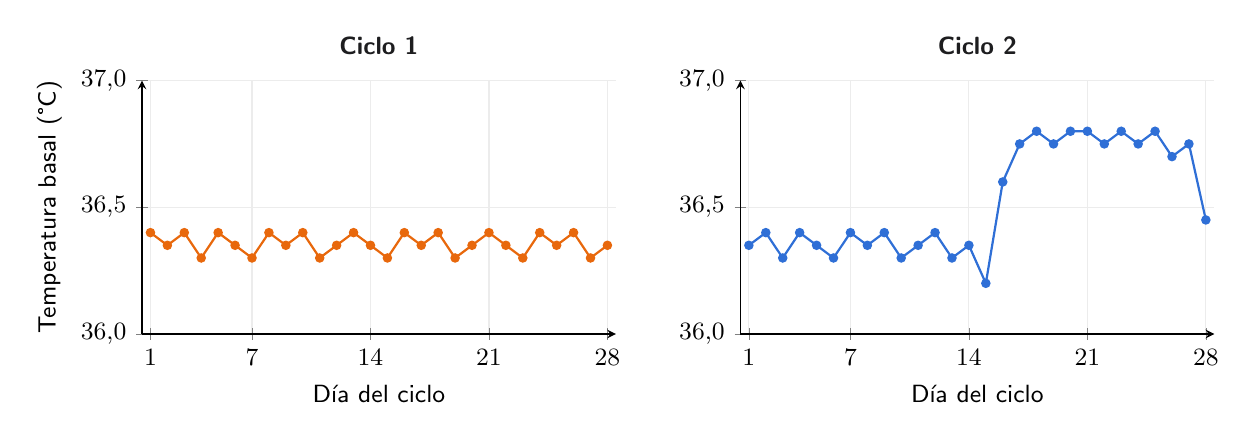
\begin{tikzpicture}[font=\small]
\pgfplotsset{t/.style={width=7.6cm,height=4.8cm,xmin=0.5,xmax=28.5,ymin=36.0,ymax=37.0,axis lines=left,xtick={1,7,14,21,28},
 ytick={36.0,36.5,37.0},yticklabel style={/pgf/number format/fixed,/pgf/number format/precision=1,/pgf/number format/fixed zerofill},
 xlabel={Día del ciclo},grid=major,grid style={gray!15},title style={font=\small\bfseries,text=tinta}}}
\begin{axis}[t,title={Ciclo 1},ylabel={Temperatura basal (°C)}]
\addplot[nar,thick,mark=*,mark size=1.3pt] coordinates {(1,36.4)(2,36.35)(3,36.4)(4,36.3)(5,36.4)(6,36.35)(7,36.3)(8,36.4)(9,36.35)(10,36.4)(11,36.3)(12,36.35)(13,36.4)(14,36.35)(15,36.3)(16,36.4)(17,36.35)(18,36.4)(19,36.3)(20,36.35)(21,36.4)(22,36.35)(23,36.3)(24,36.4)(25,36.35)(26,36.4)(27,36.3)(28,36.35)};
\end{axis}
\begin{axis}[t,title={Ciclo 2},at={(7.6cm,0)}]
\addplot[azul,thick,mark=*,mark size=1.3pt] coordinates {(1,36.35)(2,36.4)(3,36.3)(4,36.4)(5,36.35)(6,36.3)(7,36.4)(8,36.35)(9,36.4)(10,36.3)(11,36.35)(12,36.4)(13,36.3)(14,36.35)(15,36.2)(16,36.6)(17,36.75)(18,36.8)(19,36.75)(20,36.8)(21,36.8)(22,36.75)(23,36.8)(24,36.75)(25,36.8)(26,36.7)(27,36.75)(28,36.45)};
\end{axis}
\end{tikzpicture}
\end{document}
